\documentclass[11pt]{scrartcl}
\usepackage[sexy]{{style_files/evan}}

\usepackage{{style_files/NMC}}
\usepackage{standalone}
\usepackage{import}

\begin{document}
\title{NMC Problem Set \#6}
\date{Sep. 25, 2022} 
\maketitle

\section*{Welcome!}

This is a selection of interesting problems derived from curious thoughts, curated so you can nibble on them throughout the week! The point of this document is to introduce you to fun puzzles that require thinking. We recommend you try the ones that you find interesting! Feel free to work on them with others (even us teachers!). Harder problems are marked with chilies (\fullchili), in case you want to challenge yourself.
\newline\newline
Have fun! \textit{Note: New variants on these problems may be released throughout the week. Remember to check back once in a while!}
    
\section{Algebra}
\begin{enumerate}[label=\textbf{A\arabic*}.]
    \item \textbf{Functional Showdown} (Frog stylie!) \newline
    Welcome to functional showdown! This problem is divided into matches. In each match, two functions will be shown, and you will have to pick which one \textit{grows faster} than the other. A function $f$ is said to \textit{grow faster} than another function $g$ if it's "eventually bigger", as in, there is some number $C$ such that $f(x) > g(x)$ for all integers $x>C$. \newline
    It's not enough to guess which one grows faster, you also need to \emph{prove it}. That's all, have fun! 
    \begin{enumerate}
        \item Which one grows faster? One of them has a small coefficient, but a bigger exponent...
        $$\frac{1}{1000}x^2 \quad \mathbf{vs.} \quad 1000x$$
        
        \item In general, let $a,b,c,d$ be positive real numbers, when can you be sure that $cx^a$ grows faster than $dx^b$?
        
        \item Which one grows faster? Fixed exponent, or fixed base?
        $$
        6^x \ \mathbf{vs.} \ x^6, \qquad
        2^{\sqrt{x}} \ \mathbf{vs.} \ x^{20}, \qquad
        2^{\sqrt{x^x}} \ \mathbf{vs.} \ x^{2^x}, \qquad
        (8x)^{x} \ \mathbf{vs.} \ x^{8x}.
        $$
        \item We will now introduce a new operation, called \textit{factorial} ($!$). We define $x!$ as the product of all numbers up to $x$. So for example $3! = 1\cdot2\cdot3 = 6$ and $5! = 1\cdot2\cdot3\cdot3\cdot4\cdot5 = 120$.
        Which one grows faster?
        $$
        x! \ \mathbf{vs.} \ x^{100}, \qquad 
        x! \ \mathbf{vs.} \ x^x, \qquad
        x! \ \mathbf{vs.} \ x^{x/2}, \qquad
        (\text{\fullchili})\ x!\ \mathbf{vs.}\ \sqrt{2\pi x}(x/e)^x.
        $$
    \end{enumerate}
\end{enumerate}

\newpage
\section{Combinatorics}
\begin{enumerate}[label=\textbf{C\arabic*}.]
    \item \textbf{Rock, Paper, and Scissors} \newline
    Suppose $n \geq 3$ people are playing RPS. We call a game \textit{indecisive} if at least $1$ rock, paper, and scissor is played among all $n$ players, or if it ends in a tie!
    
    \begin{enumerate}
        \item What's the probability, in terms of $n$, that the game is indecisive?
        
        \item Suppose we are now playing Rock-Paper-Scissors-Lizard-Spock (RPSLS), a variant on the traditional RPS!  What's the probability that the game is indecisive assuming that $n \geq 5$?
        
        \begin{figure}[h]
            \centering
            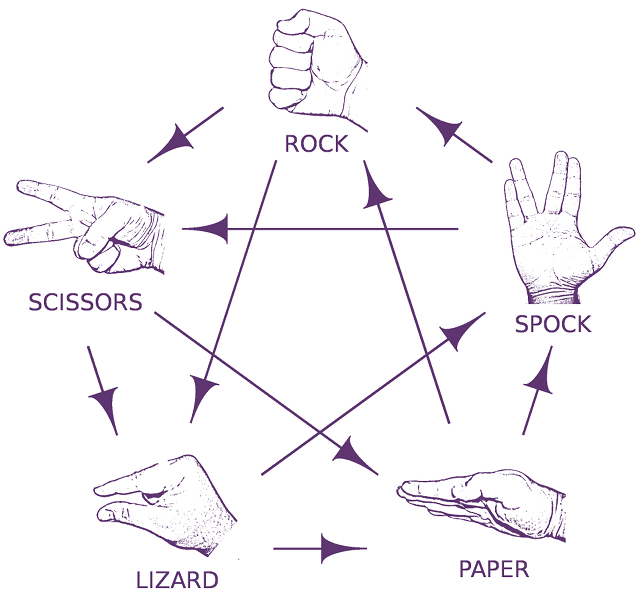
\includegraphics[width = 11cm]{Diagrams/RPSLS.png}
            \caption{Source: \href{https://puzzlewocky.com/parlor-games/rock-paper-scissors-lizard-spock/}{Thanks, puzzlewocky!}}
            \label{fig:RPSLS}
        \end{figure}
        
        \item The above diagram illustrates which move dominates which move in a game. Suppose the OneShot Math Group (4 players!) are playing a game of RPSLS \footnote{if this was according to big bang theory lore, honestly... we'll just be tie-ing over and over again because we're all boys and we only play spock. \href{https://bigbangtheory.fandom.com/wiki/Rock,_Paper,_Scissors,_Lizard,_Spock}{link to wiki}}. What's the chance that someone beats at least two other people?
    \end{enumerate}
\end{enumerate}

\newpage
\section{Geometry}
\begin{enumerate}[label=\textbf{G\arabic*}.]
    \item \textbf{Venn Diagrams} \newline
    Here, we have a Venn diagram with $3$ circles.
    \begin{figure}[h]
        \centering
        \includegraphics[width = 8cm]{Diagrams/3 Circles Venn.tex}
        \label{fig:3-Circles-Venn}
    \end{figure}
    
    We can clearly see that the regions, $\SA, \SB, \SC, \SA \cap \SB, \SA \cap \SC, \SB \cap \SC$, and $\SA \cap \SB \cap \SC$ are visible and clearly marked on this diagram.
    
    \begin{enumerate}
        \item Show that it is impossible to create a Venn diagram with circles that will represent all the possible intersections of $4$ or more sets.
        
        \item Construct a Venn diagram with congruent shapes that properly represent all possible intersections of $4$ sets.
    \end{enumerate}
\end{enumerate}

\newpage
\section{Number Theory}
\begin{enumerate}[label=\textbf{N\arabic*}.]
    \item \textbf{Periodicity} \newline
    \textit{Warning: This problem is slightly harder than our regular NT sections! It's definitely still doable if you poke at it, though. :)}
    
    In math, we call a number \textit{periodic} if its decimal expansion has a repeating pattern of terms. For example,
    \[ \frac{1}{7} = 0.\overline{142857}. \] 
    
    \begin{enumerate}
        \item Prove that the following must be true!
        \[ 0.9999\dots = 0.\overline{9} = 1. \]
        
        \item (\fullchili) If a number has a repeating or terminating decimal, must it be rational? Remember that a rational number is a fraction $p/q$ where $p, q$ are integers.
        
        \item (\fullchili) Using the idea of periodicity, prove that
        \[ \sum_{p \text{ prime}} \frac{1}{2^p} = \frac{1}{2^2} + \frac{1}{2^3} + \frac{1}{2^5} + \frac{1}{2^7} + \dots \]
        is irrational. By the same way, show that
        \[ \sum_{p \text{ prime}} \frac{1}{n^p} \not\in \QQ \text{ for } n \geq 2. \]
    \end{enumerate}
    
\end{enumerate}
\end{document}
